\documentclass{article}

\usepackage[T1]{fontenc}
\usepackage{textcomp}

\usepackage[english]{babel}
\usepackage[utf8]{inputenc}

\usepackage{lmodern}

\usepackage{hyperref}
\hypersetup{breaklinks}
\hypersetup{pdfborder=0 0 0}

\usepackage[babel=true]{microtype}

\usepackage{amsmath}

\usepackage{geometry}

\usepackage{tikz}

\usepackage[normalem]{ulem}


\title{The impact of vector interaction with other insect species on
  disease spread}

\author{
  Elizabeth Borer
  \and
  David Crowder
  \and
  Deborah Finke
  \and
  Jing Li
  \and
  Jan Medlock
  \and
  David Pattemore
  \and
  Rakefet Sharon
}


\newcommand{\md}{\mathrm{d}}
\newcommand{\me}{\mathrm{e}}
\newcommand{\mat}[1]{\mathbf{#1}}
\renewcommand{\vec}[1]{\mathbf{#1}}

\newcommand{\comment}[1]{\textbf{#1}}


\begin{document}

\maketitle

\section{Model}

Let $V_{ms}(t)$ and $V_{fs}(t)$ be the number of moving and feeding
susceptible vectors at time $t$ and $V_{mi}(t)$ and $V_{fi}(t)$ be the
number of moving and feeding infectious vectors at time $t$.
Likewise, let $P_s(t)$ and $P_i(t)$ be the number of susceptible and
infected plants at time $t$.  The total number of vectors is $V(t) =
V_{ms}(t) + V_{fs}(t) + V_{mi}(t) + V_{fi}(t)$ and the total number of
plants is $P(t) = P_s(t) + P_i(t)$.  The vectors feed on new plants at
the rate $f_V$ and spend the proportion $\phi_V$ of their time feeding
and $1 - \phi_V$ moving.  We assume that vectors only reproduce when
they are feeding; the birth rate is proportional to the number of the
feeding vectors, with a logistic term dependent on the total number of
vectors; and the newborns join the moving group.  Moving and feeding
vectors die but at different rates, with moving vectors assumed to die
more quickly than feeding vectors (i.e.~$\delta_V > 0$).

The model is
\begin{equation}
  \label{odesystem}
  \begin{split}
    \frac{\md V_{ms}(t)}{\md t}
    &=
    - \underbrace{\frac{f_V}{1 - \phi_V} V_{ms}}_\text{to feeding}
    + \underbrace{\frac{f_V}{\phi_V}  V_{fs}}_\text{from feeding}
    + \underbrace{\gamma_V V_{mi}}_\text{loss of pathogen}
    - \underbrace{(1 + \delta_V) \mu_V V_{ms}}_\text{death}
    + \underbrace{b_V V_f \left(1 - \frac{V}{K_V P}\right)}_\text{birth},
    \\
    \frac{\md V_{fs}(t)}{\md t}
    &=
    - \underbrace{\beta_V \frac{P_i}{P} V_{fs}}_\text{infection}
    + \underbrace{\frac{f_V}{1 - \phi_V} V_{ms}}_\text{from moving}
    - \underbrace{\frac{f_V}{\phi_V} V_{fs}}_\text{to moving}
    + \underbrace{\gamma_V V_{fi}}_\text{loss of pathogen}
    - \underbrace{\mu_V V_{fs}}_\text{death},
    \\
    \frac{\md V_{mi}(t)}{\md t}
    &=
    - \underbrace{\frac{f_V}{1 - \phi_V} V_{mi}}_\text{to feeding}
    + \underbrace{\frac{f_V}{\phi_V} V_{fi}}_\text{from feeding}
    - \underbrace{\gamma_V V_{mi}}_\text{loss of pathogen}
    - \underbrace{(1 + \delta_V) \mu_V V_{mi}}_\text{death},
    \\
    \frac{\md V_{fi}(t)}{\md t}
    &=
    \underbrace{\beta_V \frac{P_i}{P} V_{fs}}_\text{infection}
    + \underbrace{\frac{f_V}{1 - \phi_V} V_{mi}}_\text{from moving}
    - \underbrace{\frac{f_V}{\phi_V} V_{fi}}_\text{to moving}
    - \underbrace{\gamma_V V_{fi}}_\text{loss of pathogen}
    - \underbrace{\mu_V V_{fi}}_\text{death},
    \\
    \frac{\md P_s(t)}{\md t}
    &=
    - \underbrace{\beta_P V_{fi} \frac{P_s}{P}}_\text{infection}
    +\underbrace{\gamma_P P_i}_\text{loss of pathogen},
    \\
   \frac{\md P_i(t)}{\md t}
    &=
    \underbrace{\beta_P V_{fi} \frac{P_s}{P}}_\text{infection}
    - \underbrace{\gamma_P P_i}_\text{loss of pathogen},
  \end{split}
\end{equation}
where the number of feeding vectors is $V_f = V_{fs} + V_{fi}$,
$\beta_V$ is the infection rate from plants to vectors, $\beta_P$ is
the infection rate from vectors to plants, $\gamma_V$ is the rate of
pathogen clearance in vectors, $\mu_V$ is the death rate of the
feeding vectors, $\delta_V$ is the proportional increase in the death
rate for moving vectors, $b_V$ is the birth rate of vectors, and $K_V$
is the carrying capacity of vectors per plant
(\autoref{fig:full_model_diagram}).


\begin{figure}
  \centering
  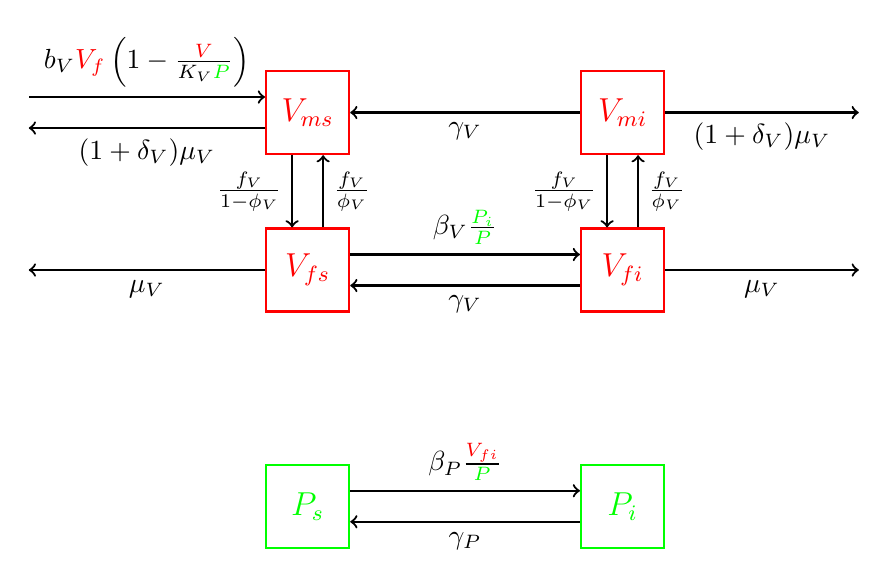
\begin{tikzpicture}[
    thick,
    scale = 1,
    compartment/.style = {draw,
      font = \large,
      minimum size = {3em}},
    plant/.style = {green},
    vector/.style = {red},
    ]

    \node at (0, 5)
    [compartment, vector, name = V_ms] {$V_{ms}$};
    \node at (4, 5)
    [compartment, vector, name = V_mi] {$V_{mi}$};

    \node at (0, 3)
    [compartment, vector, name = V_fs] {$V_{fs}$};
    \node at (4, 3)
    [compartment, vector, name = V_fi] {$V_{fi}$};

    \node at (0, 0)
    [compartment, plant, name = P_s] {$P_s$};
    \node at (4, 0)
    [compartment, plant, name = P_i] {$P_i$};

    \draw [->] (P_s.20) to node [above]
    {$\beta_P \frac{\textcolor{red}{V_{fi}}}{\textcolor{green}{P}}$}
    (P_i.160);

    \draw [->] (P_i.200) to node [below] {$\gamma_P$} (P_s.340);

    \draw [->] (V_fs.20) to node [above]
    {$\beta_V \frac{\textcolor{green}{P_i}}{\textcolor{green}{P}}$}
    (V_fi.160);

    \draw [->] (V_fi.200) to node [below] {$\gamma_V$} (V_fs.340);
    \draw [->] (V_mi) to node [below] {$\gamma_V$} (V_ms);

    \draw [->] (V_ms.250) to node [left] {$\frac{f_V}{1 - \phi_V}$} (V_fs.110);
    \draw [->] (V_mi.250) to node [left] {$\frac{f_V}{1 - \phi_V}$} (V_fi.110);

    \draw [->] (V_fs.70) to node [right] {$\frac{f_V}{\phi_V}$} (V_ms.290);
    \draw [->] (V_fi.70) to node [right] {$\frac{f_V}{\phi_V}$} (V_mi.290);

    \draw [<-] (V_ms.160) to node [above]
    {$b_V \textcolor{red}{V_f}
      \left(1 - \frac{\textcolor{red}{V}}{K_V \textcolor{green}{P}}\right)$}
    +(180: 3);

    \draw [->] (V_fs.180) to node [below] {$\mu_V$} +(180: 3);
    \draw [->] (V_ms.200) to node [below] {$(1 + \delta_V) \mu_V$} +(180: 3);

    \draw [->] (V_fi) to node [below] {$\mu_V$} +(0: 3);
    \draw [->] (V_mi) to node [below] {$(1 + \delta_V) \mu_V$} +(0: 3);
  \end{tikzpicture}
  \caption{Model diagram.  $P_s$ and $P_i$ (green) are the numbers
    of uninfected and plants.  $V_{ms}$, $V_{fs}$, $V_{mi}$, and
    $V_{fi}$ (red) are numbers of moving uninfected, feeding
    uninfected, moving infected, and feeding infected vectors.}
  \label{fig:full_model_diagram}
\end{figure}


We considered two different scenarios, one for a persistent virus and
one for a non-persistent virus (\autoref{params}).


\begin{table}
  \centering
  \begin{tabular}{llr}
    \multicolumn{2}{l}{\textbf{Parameter}}
    & \multicolumn{1}{r}{\textbf{Value}}
    \\
    $f_V$ & Rate of vectors feeding on new plants & $6\;\text{d}^{-1}$
    \\
    $\phi_V$ & Proportion of vectors' time spent feeding & $0.5$
    \\
    $\mu_V$ & Mortality rate for feeding vectors & $0.02\;\text{d}^{-1}$
    \\
    $\delta_V$ & Relative mortality increase for moving vectors & $1$
    \\
    $b_V$ & Fecundity of feeding vectors & $0.08\;\text{d}^{-1}$
    \\
    $K_V$ & Carrying capacity of vectors per plant & $100$
    \\
    $\gamma_P$ & Rate of pathogen clearance in plants & $0\;\text{d}^{-1}$
    \\
    $V(0)$ & Initial number vectors & $100$
    \\
    $P(0)$ & Initial number of plants & $10\,000$
    \\
    \multicolumn{3}{c}{\textbf{Persistent}}
    \\
    $\beta_V$ & Transmission rate from plants to vectors & $0.48\;\text{d}^{-1}$
    \\
    $\beta_P$ & Transmission rate from vectors to plants & $0.48\;\text{d}^{-1}$
    \\
    $\gamma_V$ & Rate of pathogen clearance in vectors & $0\;\text{d}^{-1}$
    \\
    \multicolumn{3}{c}{\textbf{Non-persistent}}
    \\
    $\beta_V$ & Transmission rate from plants to vectors & $4.8\;\text{d}^{-1}$
    \\
    $\beta_P$ & Transmission rate from vectors to plants & $4.8\;\text{d}^{-1}$
    \\
    $\gamma_V$ & Rate of pathogen clearance in vectors & $0.12\;\text{d}^{-1}$
  \end{tabular}
  \caption{Model parameters and initial conditions.}
  \label{params}
\end{table}


The intrinsic growth rate of the pathogen was found using numerical
solutions of ODE system \eqref{odesystem}.  The model at the
disease-free state, solved numerically for $150\;\mathrm{d}$, and the
dominant eigenvalue of the Jacobian of the ODE system was found
numerically (\autoref{fig:growth_rates}).

\section{Results}

\begin{itemize}
\item The pathogen grows slowly until the vector population becomes
  large (\autoref{fig:solutions}).

\item The pathogen growth rate increases as the vector population
  grows (\autoref{fig:growth_rates}).

\item The growth rate is insensitive to the feeding rate
  (\hyperref[fig:sensitivity_1param]{Figures
    \ref*{fig:sensitivity_1param}}--\ref{fig:sensitivity_2params}).
\end{itemize}


\begin{figure}
  \centering
  \includegraphics[width = \textwidth]{solutions}
  \caption{Model solutions for persistent and non-persistent
    scenarios.  The curves for $V_{ms}$ and $V_{mi}$ lie under the
    curves for $V_{fs}$ and $V_{fi}$ for the persistent scenario.
    Parameter values are given in \autoref{params}.
    For initial conditions, we used the result from the quasi-steady
    state approximation (\autoref{sec:QSSA}) that $50\%$ of the
    vectors are moving and $50\%$ are feeding for our parameter
    values, and that 1 of the moving vectors are infected and all
    others are uninfected ($V_{ms}(0) = 49, V_{mi}(0) = 1, V_{fs}(0) =
    50, V_{fi}(0) = 0$).}
  \label{fig:solutions}
\end{figure}

\begin{figure}
  \centering
  \includegraphics[width = \textwidth]{growth_rates}
  \caption{Intrinsic growth rate of the pathogen.  Model initial
    conditions were the disease-free state given by the parameters
    (\autoref{params}) and the result from the quasi-steady state
    approximation (\autoref{sec:QSSA}) that $50\%$ of the vectors are
    moving and $50\%$ are feeding for our parameter values ($V_{ms}(0)
    = V_{fs}(0) = 50, P_s(0) = 10\,000, V_{mi}(0) = V_{fi}(0) = P_i(0)
    = 0$).}
  \label{fig:growth_rates}
\end{figure}

\begin{figure}
  \centering
  \includegraphics[width = \textwidth]{sensitivity_1param}
  \caption{Intrinsic growth rate of the pathogen vs.~parameter values
    at $150~\text{d}$, relative to its value for the baseline
    parameter value.  The dotted horizontal lines show the baseline
    parameter values.  Parameter values and initial conditions are as
    in \autoref{fig:growth_rates}.}
  \label{fig:sensitivity_1param}
\end{figure}

\begin{figure}
  \centering
  \includegraphics[width = \textwidth]{sensitivity_1param_fV}
  \caption{Intrinsic growth rate of the pathogen vs.~the feeding rate
    ($f_V$) at $150~\text{d}$, relative to its value for the baseline
    parameter value.  The vertical axis has a linear scale, compared
    to a log scale in \autoref{fig:growth_rates}, to show the smaller
    differences in growth rate as feeding rate varies.  The dotted
    horizontal lines show the baseline parameter values.  Parameter
    values and initial conditions are as in
    \autoref{fig:growth_rates}.
    \comment{The curves do not quite go to 0 at $f_V = 0$ because
      the model assumes that feeding infected vectors are well mixed
      on the plants.  The fix is to keep track of whether vectors are
      on infected or uninfected plants.  It does not seem worth it for
      our purposes.}}
  \label{fig:sensitivity_1param_fV}
\end{figure}

\begin{figure}
  \centering
  \includegraphics[width = \textwidth]{sensitivity_2params}
  \caption{Intrinsic growth rate of the pathogen vs.~parameter values
    at $150~\text{d}$, relative to its value for the baseline
    parameter value.  Parameter values and
    initial conditions are as in \autoref{fig:growth_rates}.}
  \label{fig:sensitivity_2params}
\end{figure}


\clearpage
\appendix
\section{Quasi-steady state approximation}
\label{sec:QSSA}

To simplify the model for further analysis, we make the approximation
is that vectors switching from feeding to moving and vice versa
happens very quickly relative to birth, death, and infection, so that
the fraction of vectors moving and the fraction feeding quickly
approach a quasi-steady state as the other processes happen more
slowly.  Formally, we want $f_V \to \infty$, with
all the other parameters not large: i.e.~let $\epsilon =
\frac{1}{f_V} \to 0$ and all the other parameters
$\operatorname{O}(1)$.  From
\eqref{odesystem},
\begin{equation}
  \begin{split}
    \frac{1}{f_V} \frac{\md V_{ms}}{\md t}
    &=
    - \frac{1}{1 - \phi_V} V_{ms}
    + \frac{1}{\phi_V}  V_{fs}
    + \frac{\gamma_V}{f_V} V_{mi}
    - \frac{(1 + \delta_V) \mu_V}{f_V} V_{ms}
    + \frac{b_V}{f_V} V_f \left(1 - \frac{V}{K_V P}\right),
    \\
    \frac{1}{f_V} \frac{\md V_{mi}}{\md t}
    &=
    - \frac{1}{1 - \phi_V} V_{mi}
    + \frac{1}{\phi_V} V_{fi}
    - \frac{\gamma_V}{f_V} V_{mi}
    - \frac{(1 + \delta_V) \mu_V}{f_V} V_{ms},
  \end{split}
\end{equation}
as $\epsilon = \frac{1}{f_V} \to 0$ gives
\begin{equation}
  \begin{split}
    0 &= - \frac{1}{1 - \phi_V} V_{ms} + \frac{1}{\phi_V} V_{fs} + \mathrm{O}(\epsilon),
    \\
    0 &= - \frac{1}{1 - \phi_V} V_{mi} + \frac{1}{\phi_V} V_{fi} + \mathrm{O}(\epsilon),
  \end{split}
\end{equation}
so that
\begin{equation}
  \begin{split}
    V_{ms} &= \frac{1 - \phi_V}{\phi_V} V_{fs},
    \\
    V_{mi} &= \frac{1 - \phi_V}{\phi_V} V_{fi}.
  \end{split}
\end{equation}
to zeroth order in $\epsilon$.  If we define the numbers of
susceptible and infected vectors to be $V_s = V_{ms} + V_{fs}$ and
$V_i = V_{mi} + V_{fi}$, then
\begin{equation}
  \label{QSSA}
  \begin{aligned}
    V_{ms} &= (1 - \phi_V) V_s,
    & \quad\quad\quad\quad
    V_{fs} &= \phi_V V_s,
    \\
    V_{mi} &= (1 - \phi_V) V_i,
    &
    V_{fi} &= \phi_V V_i.
  \end{aligned}
\end{equation}
That the fractions feeding and moving in the susceptible and infected
classes follow \eqref{QSSA} is the quasi-steady-state approximation
(QSSA).

Adding the differential equations for $V_s = V_{ms} + V_{fs}$ and $V_i
= V_{mi} + V_{fi}$ gives
\begin{equation}
  \begin{split}
    \frac{\md V_s}{\md t}
    &=
    - \beta_V \frac{P_i}{P} V_{fs}
    + \gamma_V V_i
    - \mu_V V_s
    - \delta_V \mu_V V_{ms}
    + b_V V_f \left(1 - \frac{V}{K_V P}\right),
    \\
    \frac{\md V_i}{\md t}
    &=
    \beta_V \frac{P_i}{P} V_{fs}
    - \gamma_V V_i
    - \mu_V V_i
    - \delta_V \mu_V V_{mi},
    \\
    \frac{\md P_s}{\md t}
    &=
    - \beta_P V_{fi} \frac{P_s}{P}
    + \gamma_P P_i,
    \\
   \frac{\md P_i}{\md t}
    &=
    \beta_P V_{fi} \frac{P_s}{P} - \gamma_P P_i.
  \end{split}
\end{equation}
Using the QSSA \eqref{QSSA} gives
\begin{equation}
  \label{odesystem_QSSA}
  \begin{split}
    \frac{\md V_s}{\md t}
    &=
    - \overline{\beta}_V \frac{P_i}{P} V_s
    + \gamma_V V_i
    - \overline{\mu}_V V_s
    + \overline{b}_V V \left(1 - \frac{V}{K_V P}\right),
    \\
    \frac{\md V_i}{\md t}
    &=
    \overline{\beta}_V \frac{P_i}{P} V_s
    - \gamma_V V_i
    - \overline{\mu}_V V_i,
    \\
    \frac{\md P_s}{\md t}
    &=
    - \overline{\beta}_P V_{i} \frac{P_s}{P}
    + \gamma_P P_i,
    \\
    \frac{\md P_i}{\md t}
    &=
    \overline{\beta}_P V_{i} \frac{P_s}{P}
    - \gamma_P P_i,
  \end{split}
\end{equation}
where the average transmission, birth, and death rates are
\begin{equation}
  \begin{split}
    \overline{\beta}_V &= \beta_V \phi_V,
    \\
    \overline{\beta}_P &= \beta_P \phi_V,
    \\
    \overline{b}_V &= b_V \phi_V,
    \\
    \overline{\mu}_V &= \mu_V [1 + \delta_V (1 - \phi_V)].
  \end{split}
\end{equation}
(See also \autoref{fig:QSSA_model_diagram}.)


\begin{figure}
  \centering
  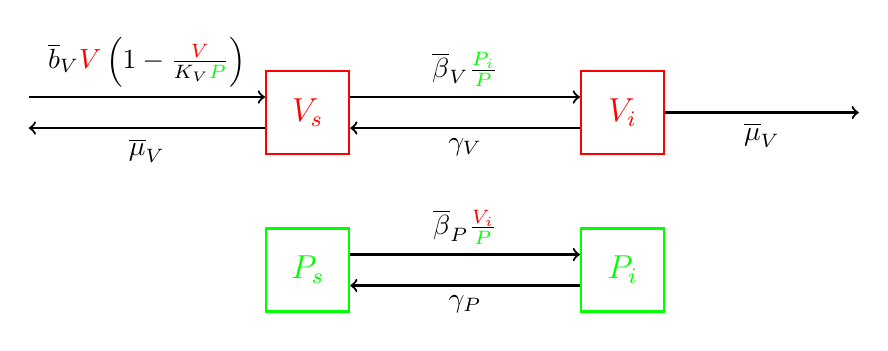
\begin{tikzpicture}[
    thick,
    scale = 1,
    compartment/.style = {draw,
      font = \large,
      minimum size = {3em}},
    plant/.style = {green},
    vector/.style = {red},
    ]

    \node at (0, 2)
    [compartment, vector, name = V_s] {$V_s$};
    \node at (4, 2)
    [compartment, vector, name = V_i] {$V_i$};

    \node at (0, 0)
    [compartment, plant, name = P_s] {$P_s$};
    \node at (4, 0)
    [compartment, plant, name = P_i] {$P_i$};

    \draw [->] (P_s.20) to node [above]
    {$\overline{\beta}_P \frac{\textcolor{red}{V_{i}}}{\textcolor{green}{P}}$}
    (P_i.160);

    \draw [->] (P_i.200) to node [below] {$\gamma_P$} (P_s.340);

    \draw [->] (V_s.20) to node [above]
    {$\overline{\beta}_V \frac{\textcolor{green}{P_i}}{\textcolor{green}{P}}$}
    (V_i.160);

    \draw [->] (V_i.200) to node [below] {$\gamma_V$} (V_s.340);

    \draw [<-] (V_s.160) to node [above]
    {$\overline{b}_V \textcolor{red}{V}
      \left(1 - \frac{\textcolor{red}{V}}{K_V \textcolor{green}{P}}\right)$}
    +(180: 3);

    \draw [->] (V_s.200) to node [below] {$\overline{\mu}_V$} +(180: 3);

    \draw [->] (V_i) to node [below] {$\overline{\mu}_V$} +(0: 3);

  \end{tikzpicture}
  \caption{QSSA model diagram.  $P_s$ and $P_i$ (green) are the
    numbers of uninfected and plants.  $V_s$ and $V_i$ (red) are
    numbers of uninfected and infected vectors.  The
    quasi-steady-state approximation (QSSA) is that rate of feeding of
    new plants ($f_V$) is very fast relative to the other transition
    rates.  This QSSA was used to simplify the full model
    (\autoref{fig:full_model_diagram}).  Overbars denote weighted
    averages of parameters over moving and feeding vectors.}
  \label{fig:QSSA_model_diagram}
\end{figure}


At the disease-free state, $V_i = P_i = 0$, $P_s = P$, and the number
of susceptible vectors is given by
\begin{equation}
  \begin{split}
    \frac{\md V_s}{\md t}
    &=
    - \overline{\mu}_V V_s
    + \overline{b}_V V_s \left(1 - \frac{V_s}{K_V P}\right),
  \end{split}
\end{equation}
which has solution
\begin{equation}
  V_s(t) =
  \frac{V_0 \; \me^{\left(\overline{b}_V - \overline{\mu}_V\right) t}}
  {1 + \frac{V_0}{V_{\infty}}
    \left[\me^{\left(\overline{b}_V - \overline{\mu}_V\right) t} - 1\right]},
\end{equation}
where
\begin{equation}
  V_{\infty} = \left(1 - \frac{\overline{\mu}_V}{\overline{b}_V}\right) K_V P.
\end{equation}
This makes apparent the characteristic time for growth of the vector
population,
\begin{equation}
  T_V = \frac{1}{\overline{b}_V - \overline{\mu}_V}.
\end{equation}
So that the no-vectors solution to be unstable, we assume that
\begin{equation}
  \overline{b}_V > \overline{\mu}_V,
\end{equation}
which is
\begin{equation}
  b_V > \frac{1 + \delta_V (1 - \phi_V)}{\phi_V} \mu_V.
\end{equation}
($K_V = \infty$ and $\overline{b}_V = \overline{\mu}_V$ are also
sufficient.)

\section{Basic reproduction number ($R_0$)}

\subsection{Full model}

The infected states are
\begin{equation}
  \label{eq:9}
  \vec{x} =
  \begin{pmatrix}
    V_{mi}
    \\
    V_{fi}
    \\
    P_i
  \end{pmatrix}.
\end{equation}
The flow of new infections and the remaining transition flows are
\begin{align}
  \mathcal{F}
  &=
  \begin{pmatrix}
    0
    \\
    0
    \\
    \beta_P V_{fi} \frac{P_s}{P}
  \end{pmatrix},
  &
  \mathcal{V}
  &=
  \begin{pmatrix}
    \left[
      \frac{f_V}{1 - \phi_V}
      + \gamma_V
      + (1 + \delta_V) \mu_V
    \right] V_{mi}
    - \frac{f_V}{\phi_V} V_{fi}
    \\
    - \frac{f_V}{1 - \phi_V} V_{mi}
    + \left(\frac{f_V}{\phi_V} + \gamma_V + \mu_V\right) V_{fi}
    - \beta_V \frac{P_i}{P} V_{fs}(t)
    \\
    \gamma_P P_i
  \end{pmatrix}.
\end{align}
Linearizing at the disease-free state,
\begin{align}
  \mat{F} &=
  \begin{bmatrix}
    0
    &
    0
    &
    0
    \\
    0
    &
    0
    &
    0
    \\
    0
    &
    \beta_P
    &
    0
  \end{bmatrix},
  &
  \mat{V} &=
  \begin{bmatrix}
    \frac{f_V}{1 - \phi_V} + \gamma_V + (1 + \delta_V) \mu_V
    &
    - \frac{f_V}{\phi_V} 
    &
    0
    \\
    - \frac{f_V}{1 - \phi_V}
    &
    \frac{f_V}{\phi_V} + \gamma_V + \mu_V
    &
    - \beta_V \frac{V_{fs}(t)}{P}
    \\
    0
    &
    0
    &
    \gamma_P
  \end{bmatrix}.
\end{align}
The residence times are
\begin{equation}
  \mat{V}^{-1} =
  \begin{bmatrix}
    D_{V_m} & s_{V_f} D_{V_m}
    & \beta_V \frac{V_{fs}(t)}{P} D_P s_{V_f} D_{V_m}
    \\
    s_{V_m} D_{V_f} & D_{V_f}
    & \beta_V \frac{V_{fs}(t)}{P} D_P D_{V_f}
    \\
    0 & 0 & D_P
  \end{bmatrix},
\end{equation}
where the durations of one bout of moving and feeding respectively are
\begin{align}
  d_{V_m} &= \frac{1}{\frac{f_V}{1 - \phi_V} + \gamma_V + (1 + \delta_V) \mu_V}
  & \text{and} & &
  d_{V_f} &= \frac{1}{\frac{f_V}{\phi_V} + \gamma_V + \mu_V};
\end{align}
the probabilities of remaining alive and infected after one of those
bouts are
\begin{align}
  s_{V_m} &= \frac{\frac{f_V}{1 - \phi_V}}{\frac{f_V}{1 - \phi_V} + \gamma_V + (1 + \delta_V) \mu_V}
  & \text{and} & &
  s_{V_f} &= \frac{\frac{f_V}{\phi_V}}{\frac{f_V}{\phi_V} + \gamma_V + \mu_V};
\end{align}
and the total times spent moving and feeding are the probabilities of
having 1, 2, 3, $\ldots$ total bouts times the durations of those
bouts,
\begin{equation}
  \begin{split}
    D_{V_m} &= d_{V_m} + s_{V_m} s_{V_f} d_{V_m}
    + \left(s_{V_m} s_{V_f}\right)^2 d_{V_m} + \cdots
    = \frac{d_{V_m}}{1 - s_{V_f} s_{V_m}},
    \\
    D_{V_f} &= d_{V_f} + s_{V_f} s_{V_m} d_{V_f}
    + \left(s_{V_f} s_{V_m}\right)^2 d_{V_f} + \cdots
    = \frac{d_{V_f}}{1 - s_{V_f} s_{V_m}};
  \end{split}
\end{equation}
and the duration of infection in plants is
\begin{equation}
  D_P = \frac{1}{\gamma_P}.
\end{equation}
The next-generation matrix is 
\begin{equation}
  \mat{G} = \mat{F} \mat{V}^{-1} =
  \begin{bmatrix}
    0 & 0 & 0 \\
    0 & 0 & 0 \\
    s_{V_m} \beta_P D_{V_f} & \beta_P D_{V_f}
    & \beta_V \frac{V_{fs}(t)}{P} D_P \beta_P D_{V_f}
  \end{bmatrix},
\end{equation}
which has largest eigenvalue
\begin{equation}
  R_0 = \beta_V \frac{V_{fs}(t)}{P} D_P \beta_P D_{V_f}.
\end{equation}
That is, starting with 1 infected plant, it transmits infection at
rate $\beta_V$ to each of the $\frac{V_{fs}(t)}{P}$ susceptible vectors
feeding on it for the duration $D_P$ of its infection, then each of
those newly infected vectors move to new plants and transmit infection
at rate $\beta_P$ to susceptible plants for the duration $D_{Vf}$ that
they are infected and feeding.

Unfortunately, we want to consider the case where plants do not
recover ($\gamma_P = 0$), which gives $R_0 = \infty$.

\subsection{QSSA model}

The infected states
\begin{equation}
  \vec{x} =
  \begin{pmatrix}
    V_i \\ P_i
  \end{pmatrix}
\end{equation}
are governed by
\begin{equation}
  \label{infectedsystem}
  \frac{\md}{\md t}
  \begin{pmatrix}
    V_i \\ P_i
  \end{pmatrix}
  =
  \begin{pmatrix}
    \overline{\beta}_V \frac{P_i}{P} V_s(t)
    - (\gamma_V + \overline{\mu}_V) V_i
    \\
    \overline{\beta}_P V_{i} \frac{P_s}{P}
    - \gamma_P P_i
  \end{pmatrix},
\end{equation}
from \eqref{odesystem_QSSA}.  From this, the flow of new plant
infections is
\begin{equation}
  \mathcal{F} =
  \begin{pmatrix}
    0
    \\
    \overline{\beta}_P V_{i} \frac{P_s}{P}
  \end{pmatrix},
\end{equation}
and the remaining transition flow is
\begin{equation}
  \mathcal{V} =
  \begin{pmatrix}
    - \overline{\beta}_V \frac{P_i}{P} V_s(t)
    +(\gamma_V + \overline{\mu}_V) V_i
    \\
    \gamma_P P_i
  \end{pmatrix}.
\end{equation}
Linearizing these at the disease-free state gives
\begin{align}
  \mat{F} &=
  \begin{bmatrix}
    0 & 0
    \\
    \overline{\beta}_P & 0
  \end{bmatrix}, & \mat{V} &=
  \begin{bmatrix}
    \gamma_V + \overline{\mu}_V
    & - \overline{\beta}_V \frac{V_s(t)}{P}
    \\
    0 & \gamma_P
  \end{bmatrix},
\end{align}
so that the residence times are
\begin{equation}
  \mat{V}^{-1} =
  \begin{bmatrix}
    \frac{1}{\gamma_V + \overline{\mu}_V}
    & \frac{\overline{\beta}_V}
    {\gamma_P \left(\gamma_V + \overline{\mu}_V\right)}
    \frac{V_s(t)}{P}
    \\
    0 & \frac{1}{\gamma_P}
  \end{bmatrix},
\end{equation}
and the next-generation matrix is
\begin{equation}
  \mat{G} = \mat{F} \mat{V}^{-1}
  =
  \begin{bmatrix}
    0 & 0
    \\
    \frac{\overline{\beta}_P}{\gamma_V + \overline{\mu}_V}
    &
    \frac{\overline{\beta}_P \overline{\beta}_V}
    {\gamma_P \left(\gamma_V + \overline{\mu}_V\right)}
    \frac{V_s(t)}{P}
  \end{bmatrix}.
\end{equation}
The dominant eigenvalue of $\mat{G}$ is
\begin{equation}
  \label{R0QSSA}
  R_0 =
  \frac{\overline{\beta}_P \overline{\beta}_V}
  {\gamma_P \left(\gamma_V + \overline{\mu}_V\right)}
  \frac{V_s(t)}{P}.
\end{equation}


\section{Intrinsic growth rate ($r_0$)}

\subsection{Full model}

The flows for the infected states are
\begin{equation}
  \frac{\md}{\md t}
  \begin{pmatrix}
    V_{mi}
    \\
    V_{fi}
    \\
    P_i
  \end{pmatrix}
  =
  \begin{pmatrix}
    - \frac{f_V}{1 - \phi_V} V_{mi}
    + \frac{f_V}{\phi_V} V_{fi}
    - \gamma_V V_{mi}
    - (1 + \delta_V) \mu_V V_{mi}
    \\
    \beta_V \frac{P_i}{P} V_{fs}(t)
    + \frac{f_V}{1 - \phi_V} V_{mi}
    - \frac{f_V}{\phi_V} V_{fi}
    - \gamma_V V_{fi}
    - \mu_V V_{fi}
    \\
    \beta_P V_{fi} \frac{P_s}{P}
    - \gamma_P P_i
  \end{pmatrix}.
\end{equation}
The Jacobian at the disease-free state is
\begin{equation}
  \mat{J} =
  \begin{bmatrix}
    - \left[
      \frac{f_V}{1 - \phi_V}
      + \gamma_V + (1 + \delta_V) \mu_V
    \right]
    &
    \frac{f_V}{\phi_V}
    &
    0
    \\
    \frac{f_V}{1 - \phi_V}
    &
    - (\frac{f_V}{\phi_V} + \gamma_V + \mu_V)
    &
    \beta_V \frac{V_{fs}(t)}{P}
    \\
    0
    &
    \beta_P
    &
    - \gamma_P
  \end{bmatrix}.
\end{equation}
The largest eigenvalue of $\mat{J}$ is the infection growth rate
$r_0$.  Unfortunately, the characteristic equation for $\mat{J}$ is a
proper cubic,
\begin{equation}
  r_0^3 + A r_0^2 + B r_0 + C = 0,
\end{equation}
with
\begin{equation}
  \begin{split}
    A &= \frac{f_V}{1 - \phi_V} + \frac{f_V}{\phi_V} + 2 \gamma_V + (2 + \delta_V) \mu_V
    + \gamma_P,
    \\
    B &= \left[
      \frac{f_V}{1 - \phi_V} + \gamma_V + (1 + \delta_V) \mu_V
    \right]
    \left(\frac{f_V}{\phi_V} + \gamma_V + \mu_V + \gamma_P\right)
    + \left(\frac{f_V}{\phi_V} + \gamma_V + \mu_V\right) \gamma_P
    \\ & \quad\quad\quad {}
    - \frac{f_V^2}{\phi (1 - \phi_V)}
    - \beta_V \beta_P \frac{V_{fs}(t)}{P},
    \\
    C &= \left[
      \frac{f_V}{1 - \phi_V} + \gamma_V + (1 + \delta_V) \mu_V
    \right]
    \left[
      \left(\frac{f_V}{\phi_V} + \gamma_V + \mu_V\right) \gamma_P
      - \beta_P \beta_V \frac{V_{fs}(t)}{P}
    \right]
    - \frac{f_V^2}{\phi_V (1 - \phi_V)} \gamma_P,
  \end{split}
\end{equation}
making the solution for $r_0$ very complex.

\subsection{QSSA model}

To find the infection growth rate $r_0$, we linearize the equations for
the infected states \eqref{infectedsystem} at the disease-free
state:
\begin{align}
  \mat{J} =
  \begin{bmatrix}
    - (\gamma_V + \overline{\mu}_V)
    &
    \overline{\beta}_V \frac{V_s(t)}{P}
    \\
    \overline{\beta}_P
    &
    - \gamma_P
  \end{bmatrix},
\end{align}
which has dominant eigenvalue
\begin{equation}
  \label{rQSSA}
  r_0 = \frac{- (\gamma_P + \gamma_V + \overline{\mu}_V)
    + \sqrt{(\gamma_P + \gamma_V + \overline{\mu}_V)^2
      + 4 \left[\overline{\beta}_P \overline{\beta}_V \frac{V_s(t)}{P}
        - \gamma_P (\gamma_V + \overline{\mu}_V)\right]}}{2}.
\end{equation}

The harmonic mean over plants and vectors of the infection duration
\begin{equation}
  T_C = \frac{2}{\gamma_P + \gamma_V + \overline{\mu}_V}
\end{equation}
is a characteristic time for infection clearance.  The geometric
mean time to a new infection
\begin{equation}
  T_I =
  \frac{1}{\sqrt{\overline{\beta}_P \overline{\beta}_P
      \frac{V_s(t)}{P}
      - \gamma_P (\gamma_V + \overline{\mu}_V)}},
\end{equation}
is a the characteristic time for new infections.  We can write the
growth rate as
\begin{equation}
  r_0 = \sqrt{\frac{1}{T_C^2} + \frac{1}{T_I^2}} - \frac{1}{T_C},
\end{equation}
so then
\begin{equation}
  \begin{aligned}
    T_I &\ll T_C
    & & \implies &
    r_0 &\approx \frac{1}{T_I},
    \\
    T_I &\gg T_C
    & & \implies &
    r_0 &\approx \frac{1}{2 T_I} \frac{T_C}{T_I}.
  \end{aligned}
\end{equation}

The growth rate can be further simplified by assuming that
$V_0 \ll V_{\infty}$ and $t$ is small enough so that
\begin{equation}
  \frac{V_0}{V_\infty}
  \left[\me^{t / T_V} - 1\right]
  \ll 1,
\end{equation}
giving
\begin{equation}
  V_s(t) \approx V_0 \; \me^{t / T_V}.
\end{equation}
Thus,
\begin{equation}
  T_I
  \approx \frac{1}{\sqrt{\overline{\beta}_P \overline{\beta}_P
      \frac{V_o}{P} \me^{t / T_V}
      - \gamma_P (\gamma_V + \overline{\mu}_V)}}.
\end{equation}
For large time (with $\overline{b}_V > \overline{\mu}_V$),
\begin{equation}
  T_I \approx \frac{
    \me^{- t / 2 T_V}}
  {\sqrt{\overline{\beta}_P \overline{\beta}_P \frac{V_o}{P}}},
\end{equation}
so that eventually $T_I \ll T_C$ and
\begin{equation}
  r_0 \approx 
  \me^{t / 2 T_V}
  \sqrt{\overline{\beta}_P \overline{\beta}_P \frac{V_o}{P}}.
\end{equation}



\section{Analysis of increasing interactions}

Let $n$ be the level of interaction of the vector species with the
other insect species, with $n = 0$ being no interaction.  Initially,
we will consider just this implicit representation of the second insect
species, but later we may explicitly model this population as well.

We are initially thinking that the effects of the second insect
species will be on vector birth rate, vector death rate, vector
feeding rate, and vector proportion of time spend feeding.  We will
take these to have constant semi-elasticity:
\begin{equation}
  \begin{split}
    b_V(n) &= \hat{b}_V \exp\left(\epsilon_{\mu_V} n\right),
    \\
    \mu_V(n) &= \hat{\mu}_V \exp\left(\epsilon_{\mu_{V}} n\right),
    \\
    f_V(n) &= \hat{f}_V \exp\left(\epsilon_{f_V} n\right),
    \\
    \phi_V(n) &= \hat{\phi}_V \exp\left(\epsilon_{\phi_V} n\right).
  \end{split}
\end{equation}

\newcommand{\elasticity}[2]{\mathcal{E}_{#2}\negthickspace\left({#1}\right)}
Then
\begin{equation}
  \elasticity{r_0}{n} =
  \frac{1}{r_0} \frac{\md r_0}{\md n} =
\end{equation}


\end{document}
